\section{Weighted Decision Matrix}
\label{sec:decision_matrix}
The results from Chapter \ref{part:results} were collated for numerical comparative analysis using a weighted decision matrix. The results of each performance parameter were linearised to provide scores between 1-10. Weights were applied to each score according to the importance of the parameter to the effectiveness of a space-based ADS-B system. An aggregate score for a constellation was summed from each of the weighted scores and this was used to numerically compare different the different constellations tested.

\subsection{Parameter Weight Matrix}
Each of the four performance metrics described in Section \ref{sec:perfMetrics} were considered differently for each of the tested flight paths detailed in Section \ref{sec:flight_selection}. In addition to these, total number of satellites was also considered for evaluation of overall cost of the system. The parameters used in the weighted decision matrix are given in Table \ref{tab:parameters}

% Table generated by Excel2LaTeX from sheet 'weights'
\begin{table}[htbp]
  \centering
  \caption{Parameters used to evaluate constellation effectiveness}
    \begin{tabular}{lp{5cm}p{6cm}r}
    \toprule
    Flight Path & Parameter & Score Calculation Method & Weight \\
    \midrule
    All   & Number of Satellites & Simple Linearisation - Down  & 10\\
    LAX - Heathrow & Fraction of coverage gap to total time analysed & Simple Linearisation - Down & 20 \\
    LAX - Heathrow & Average Period & Pass-Fail Linearisation  & 10\\
    LAX - Heathrow & Periodicity Deviation & Pass-Fail Linearisation & 5 \\
    LAX - Heathrow & Maximum coverage gap time & Simple Linearisation - Down & 10 \\
    LAX - Heathrow & Minimum Received RX Power & Simple Linearisation - Up & 15 \\
    LAX - Narita & Fraction of coverage gap to total time analysed& Simple Linearisation - Down & 20 \\
    LAX - Narita & Average Period & Pass-Fail Linearisation & 10 \\
    LAX - Narita & Periodicity Deviation & Pass-Fail Linearisation & 5  \\
    LAX - Narita & Maximum coverage gap time & Simple Linearisation - Down & 10 \\
    LAX - Narita & Minimum Received RX Power & Simple Linearisation - Up & 15 \\
    LAX - Sydney & Fraction of coverage gap to total time analysed  & Simple Linearisation - Down & 20 \\
    LAX - Sydney & Average Period & Pass-Fail Linearisation & 10\\
    LAX - Sydney & Periodicity Deviation & Pass-Fail Linearisation & 5 \\
    LAX - Sydney & Maximum coverage gap time & Simple Linearisation - Down & 10\\
    LAX - Sydney & Minimum Received RX Power & Simple Linearisation - Up & 15\\
    \bottomrule
    \end{tabular}%
  \label{tab:parameters}%
\end{table}%

The weights were applied as shown in Table \ref{tab:parameters} subjectively, representing one particular design philosophy. Each flight path was weighted equally in favour evaluating each constellation without geographical bias\footnote{This could practically not be the best means of assigning bias. It was noted that the frequency and number of flights along each path differed. However geographical coverage was considered the most important factor in this case}. Fraction of coverage gap was determined to be the strongest factor as a higher score would ease the system requirements of a number of key factors, including signal collision avoidance and raw samples available. This was followed by minimum received RX power, which would be a defining system requirement for a space based ADS-B sensor. Satellite number and periodicity were less important as CubeSats are relatively cheap to launch and the effect of periodicity can be offset by having a higher access-coverage ratio. 

\subsection{Score Calculation}
  
\subsubsection{Simple Linearisation}
In order to simplify numerical analysis, the numerical results (other than periodicity) from each of experiments conducted in Part \ref{part:results} were linearised between minimum and maximum values. The direction of linearisation was adjusted such that a higher score meant a more favourable result. In the case of maximum, average and fraction of coverage gap times and number of satellites, this meant that a lower value was more favourable, resulting in the formula
\begin{align}
	\text{Linearsed score} = 10 \times \left[1 - \dfrac{\text{result} + \text{minimum}}{\text{maximum} - \text{minimum}}\right]. \label{eqn:linearisation}
\end{align}

For the minimum received RX power a higher the value was more favourable, resulting in the calculation 
\begin{align}
	\text{Linearsed score} = 10 \times \left[\dfrac{\text{result} + \text{minimum}}{\text{maximum} - \text{minimum}}\right]. \label{eqn:linearisation_up}
\end{align}

No further normalisation was applied. This allowed for a very basic comparison of a parameter for a set of constellations. 

\subsubsection{Pass - Fail Linearisation}
The score for coverage-gap periodicity was calculated using a pass - fail criteria. It was determined that a minimum, a second harmonic deviation away from the ideal straight-line flight path would need to be detected and mapped. As illustrated in Figure \ref{fig:2ndHarmonic}, this required three discrete sample points in addition to the data from the source and destination. This meant that the maximum allowable period was one quarter of the total flight time. The score was then calculated with the adjusted maximum using Equation (\ref{eqn:linearisation}), meaning that any period greater than the maximum would be a `0' or a `fail'.
\begin{figure}[H]
	\centering
	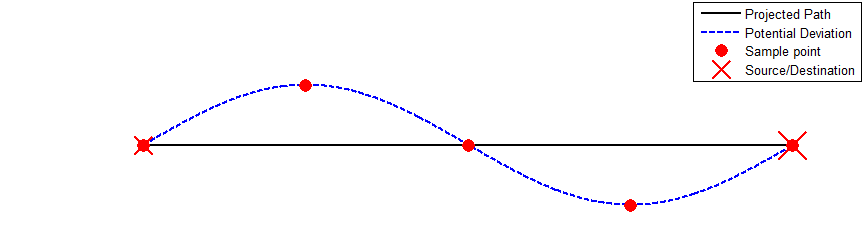
\includegraphics[scale = 0.75]{Pictures/2ndHarmonic.png}
	
	\caption{The second harmonic deviation from a straight line path, showing required sample points}
	\label{fig:2ndHarmonic}
\end{figure}
The regularity of the period was also of concern to the `sampling' ability of a given constellation. A more regular period represented a more `reliable' sampling rate and therefore a lower standard deviation of period was desired. As discussed in Section \ref{sec:periodicity_stats}, the distribution of periods which fitted a student's t distribution with an undefined standard deviation represented the greatest confidence for regularity. These cases were automatically assigned a full 10/10 score, whilst other situations with non-singular standard deviations were calculated using Equation \ref{eqn:linearisation_up} with the minimum set to `0'.

\subsection{Results}
The three highest scoring constellations, with their relative scores, are shown in Table \ref{tab:decMatRes}. The decision matrix heavily favoured the constellations with more satellites and lower altitudes. A higher number of satellites had a positive impact on the access-coverage characteristics, whilst lower altitude satellites had much more favourable potential signal strengths. A different set of results could be produced if the decision matrix were weighted according to a different set of design principles. The distribution of scores showed that most scores fell within a tight band around 70 \%, as seen in Figure \ref{fig:decisionMatrixHist}

% Table generated by Excel2LaTeX from sheet 'Sheet1'
\begin{table}[htbp]
  \centering
  \caption{The three highest scoring constellations after applying the weighted decision matrix}
    \begin{tabular}{rlrr}
    \toprule
    Case Number & Satellite Parameters &       & Score (\%) \\
    \midrule
    \multicolumn{1}{c}{\multirow{1}[10]{*}{22}} & Altitude (km above mean radius of Earth) & 700   & \multicolumn{1}{c}{\multirow{1}[10]{*}{78.45}} \\
    \multicolumn{1}{c}{} & Inclination (deg) & 60    & \multicolumn{1}{c}{} \\
    \multicolumn{1}{c}{} & Number of Planes & 3     & \multicolumn{1}{c}{} \\
    \multicolumn{1}{c}{} & Number of Satellites per plane & 6     & \multicolumn{1}{c}{} \\
    \multicolumn{1}{c}{} & Number of Satellites (Total) & 18    & \multicolumn{1}{c}{} \\ \hline
    \multicolumn{1}{c}{\multirow{1}[10]{*}{21}} & Altitude (km above mean radius of Earth) & 700   & \multicolumn{1}{c}{\multirow{1}[10]{*}{74.39}} \\
    \multicolumn{1}{c}{} & Inclination (deg) & 60    & \multicolumn{1}{c}{} \\
    \multicolumn{1}{c}{} & Number of Planes & 3     & \multicolumn{1}{c}{} \\
    \multicolumn{1}{c}{} & Number of Satellites per plane & 5     & \multicolumn{1}{c}{} \\
    \multicolumn{1}{c}{} & Number of Satellites (Total) & 15    & \multicolumn{1}{c}{} \\ \hline
    \multicolumn{1}{c}{\multirow{1}[10]{*}{1}} & Altitude (km above mean radius of Earth) & 400   & \multicolumn{1}{c}{\multirow{1}[10]{*}{73.22}} \\
    \multicolumn{1}{c}{} & Inclination (deg) & 60    & \multicolumn{1}{c}{} \\
    \multicolumn{1}{c}{} & Number of Planes & 3     & \multicolumn{1}{c}{} \\
    \multicolumn{1}{c}{} & Number of Satellites per plane & 4     & \multicolumn{1}{c}{} \\
    \multicolumn{1}{c}{} & Number of Satellites (Total) & 12    & \multicolumn{1}{c}{} \\
    \bottomrule
    \end{tabular}%
  \label{tab:decMatRes}%
\end{table}%

\begin{figure}[H]
	\centering
	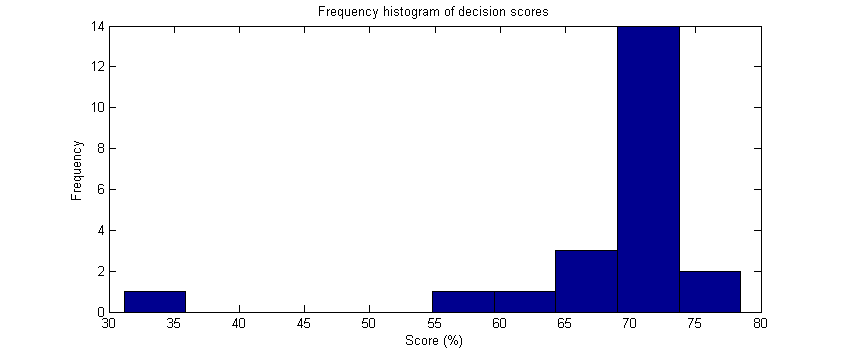
\includegraphics[scale = 0.6]{Pictures/decisionMatrixHist.png}
	
	\caption{Distribution of scores from decision matrix}
	\label{fig:decisionMatrixHist}
\end{figure}

